\documentclass[letterpaper]{article}

\usepackage{natbib,alifeconf}
\usepackage{url,hyperref,cleveref}
\usepackage{booktabs}

\newcommand\blfootnote[1]{%
  \begingroup
  \renewcommand\thefootnote{}\footnote{#1}%
  \addtocounter{footnote}{-1}%
  \endgroup
}

\title{Digital Twins for Fungal Computing: Viable XOR Regimes and Parameter Inference in Mycelial Networks}

\author{
    Anonymous Submission
}

\begin{document}

\maketitle

\begin{abstract}
Fungal substrates are promising candidates for unconventional computing, but specimen-to-specimen variability makes logic-gate fabrication difficult to reproduce. This paper presents a digital-twin workflow for fungal excitable networks and evaluates the two components needed for computer-aided design: identifying regions of parameter space that support XOR computation, and inferring latent biophysical parameters from electrical characterization data. The model represents mycelium as a random geometric graph with FitzHugh--Nagumo node dynamics and memristive edge conductances. A systematic optimization study over 160 simulated specimens identifies a viable XOR subspace defined by tuned biophysical parameters, electrode geometry, and stimulus timing. A second study applies three characterization protocols---step response, paired pulse, and triangle sweep---to 400 simulated specimens and extracts 94 response features. Random forest regressors recover some latent parameters reliably ($R^2=0.912$ for $\tau_v$, $0.816$ for $\tau_w$, $0.717$ for $a$), while others remain difficult to identify ($R^2 \approx 0$ for $v_{\text{scale}}$, $R_{\mathrm{on}}$, and $R_{\mathrm{off}}$). Protocol ablation shows that different stimulation protocols carry complementary information: step response dominates $\tau_v$, paired pulse is most informative for $a$, and step+triangle best captures $\tau_w$, $\alpha$, and $R_{\mathrm{off}}$. These results support a narrower but stronger claim than full end-to-end rediscovery: fungal digital twins are already useful for discovering viable computational regimes and for partially identifying the excitable and plastic dynamics that govern them.
\end{abstract}

Submission type: \textbf{Full Paper}\\
Data/Code available at: \url{https://anonymous.4open.science/}
\blfootnote{\textcopyright 2026 Anonymous Authors. Published under a Creative Commons Attribution 4.0 International (CC BY 4.0) license.}

\section{Introduction}
Fungal computing treats living mycelial networks as excitable, adaptive substrates for information processing \citep{adamatzky2018towards, adamatzky2022fungal, adamatzky2023fungal}. Mycelia generate structured electrical activity, respond to stimulation, and can realize logic operations through the propagation and interaction of signals in space and time \citep{adamatzky2020boolean, roberts2022mining}. They also exhibit memristive behavior, making them attractive as low-energy, self-organizing computing materials \citep{beasley2022mem, larocco2025sustainable}.

The main obstacle is variability. Different fungal specimens can differ in network topology, excitability, recovery time scales, and adaptive conductance. As a result, an electrode configuration that produces useful logic on one specimen may not transfer to another. This makes design-by-trial-and-error expensive and suggests the need for calibrated \emph{digital twins}: computational surrogates that can be probed and optimized \textit{in silico} before physical intervention. More generally, digital twins are valuable in biological systems when they support intervention planning while making clear which latent properties are actually identifiable from observations \citep{wu2024generative, clancy2026credible}.

This paper focuses on the parts of the pipeline that are already mature enough for an ALIFE full paper. First, we ask which fungal parameter regimes are viable substrates for XOR computation. Second, we ask whether standardized electrical probes contain enough information to infer the latent parameters of the model. Third, we test which characterization protocols contribute most to identifiability. A reduced rediscovery validation based on waveform matching is in progress and is included here only as a placeholder for the camera-ready version.

The contribution is therefore a computational design framework rather than a claim of fully solved twin transfer. The framework couples a biophysically motivated model, systematic logic-gate optimization, protocol-based system identification, and data-driven inverse modeling. The main result is that viable XOR behavior occupies a constrained but nontrivial region of parameter space, and that a subset of the latent parameters governing that behavior can already be recovered with useful accuracy from compact stimulation protocols.

\section{Methods}
\subsection{Fungal Network Model}
The fungal substrate is modeled as a random geometric graph in a $20 \times 20$~mm spatial domain. Nodes represent hyphal junctions and edges represent conductive hyphal connections. Each node follows FitzHugh--Nagumo excitable dynamics with fast voltage and slow recovery variables, while each edge carries a memristive state that modulates effective conductance. The full model is controlled by eight latent parameters: $\tau_v$, $\tau_w$, $a$, $b$, $v_{\text{scale}}$, $R_{\mathrm{off}}$, $R_{\mathrm{on}}$, and $\alpha$. Network size varied from 20 to 120 nodes. The implementation is described in the accompanying codebase and was simulated with adaptive ODE integration in Python.

\subsection{Viable XOR Range Discovery}
To identify parameter regimes that support logic, we ran a systematic optimization study on 160 specimens spanning eight network sizes (20 trials per size). For each specimen, Bayesian optimization searched over electrode positions, stimulus voltage, pulse duration, and inter-input delay to maximize XOR performance. A second tuning stage optimized the eight biophysical parameters while keeping the optimized gate geometry fixed. Viability was defined as membership in the top quartile of tuned XOR scores. This produces a practical ``computational prior'' over fungal parameters: a narrower range of specimens likely to support XOR-like behavior.

\subsection{Characterization Dataset}
To build an inverse model, we generated 400 simulated specimens (50 per network size across the same eight graph sizes). Each specimen was probed with three characterization protocols:
\begin{enumerate}
    \item a step response,
    \item a paired-pulse protocol at three interpulse intervals,
    \item a triangle voltage sweep.
\end{enumerate}
From these responses we extracted 94 features describing amplitude, latency, decay, facilitation/depression, hysteresis, asymmetry, nonlinearity, and smoothness. These 400 simulations provide the supervised dataset used for parameter prediction.

\begin{figure*}[t]
\centering
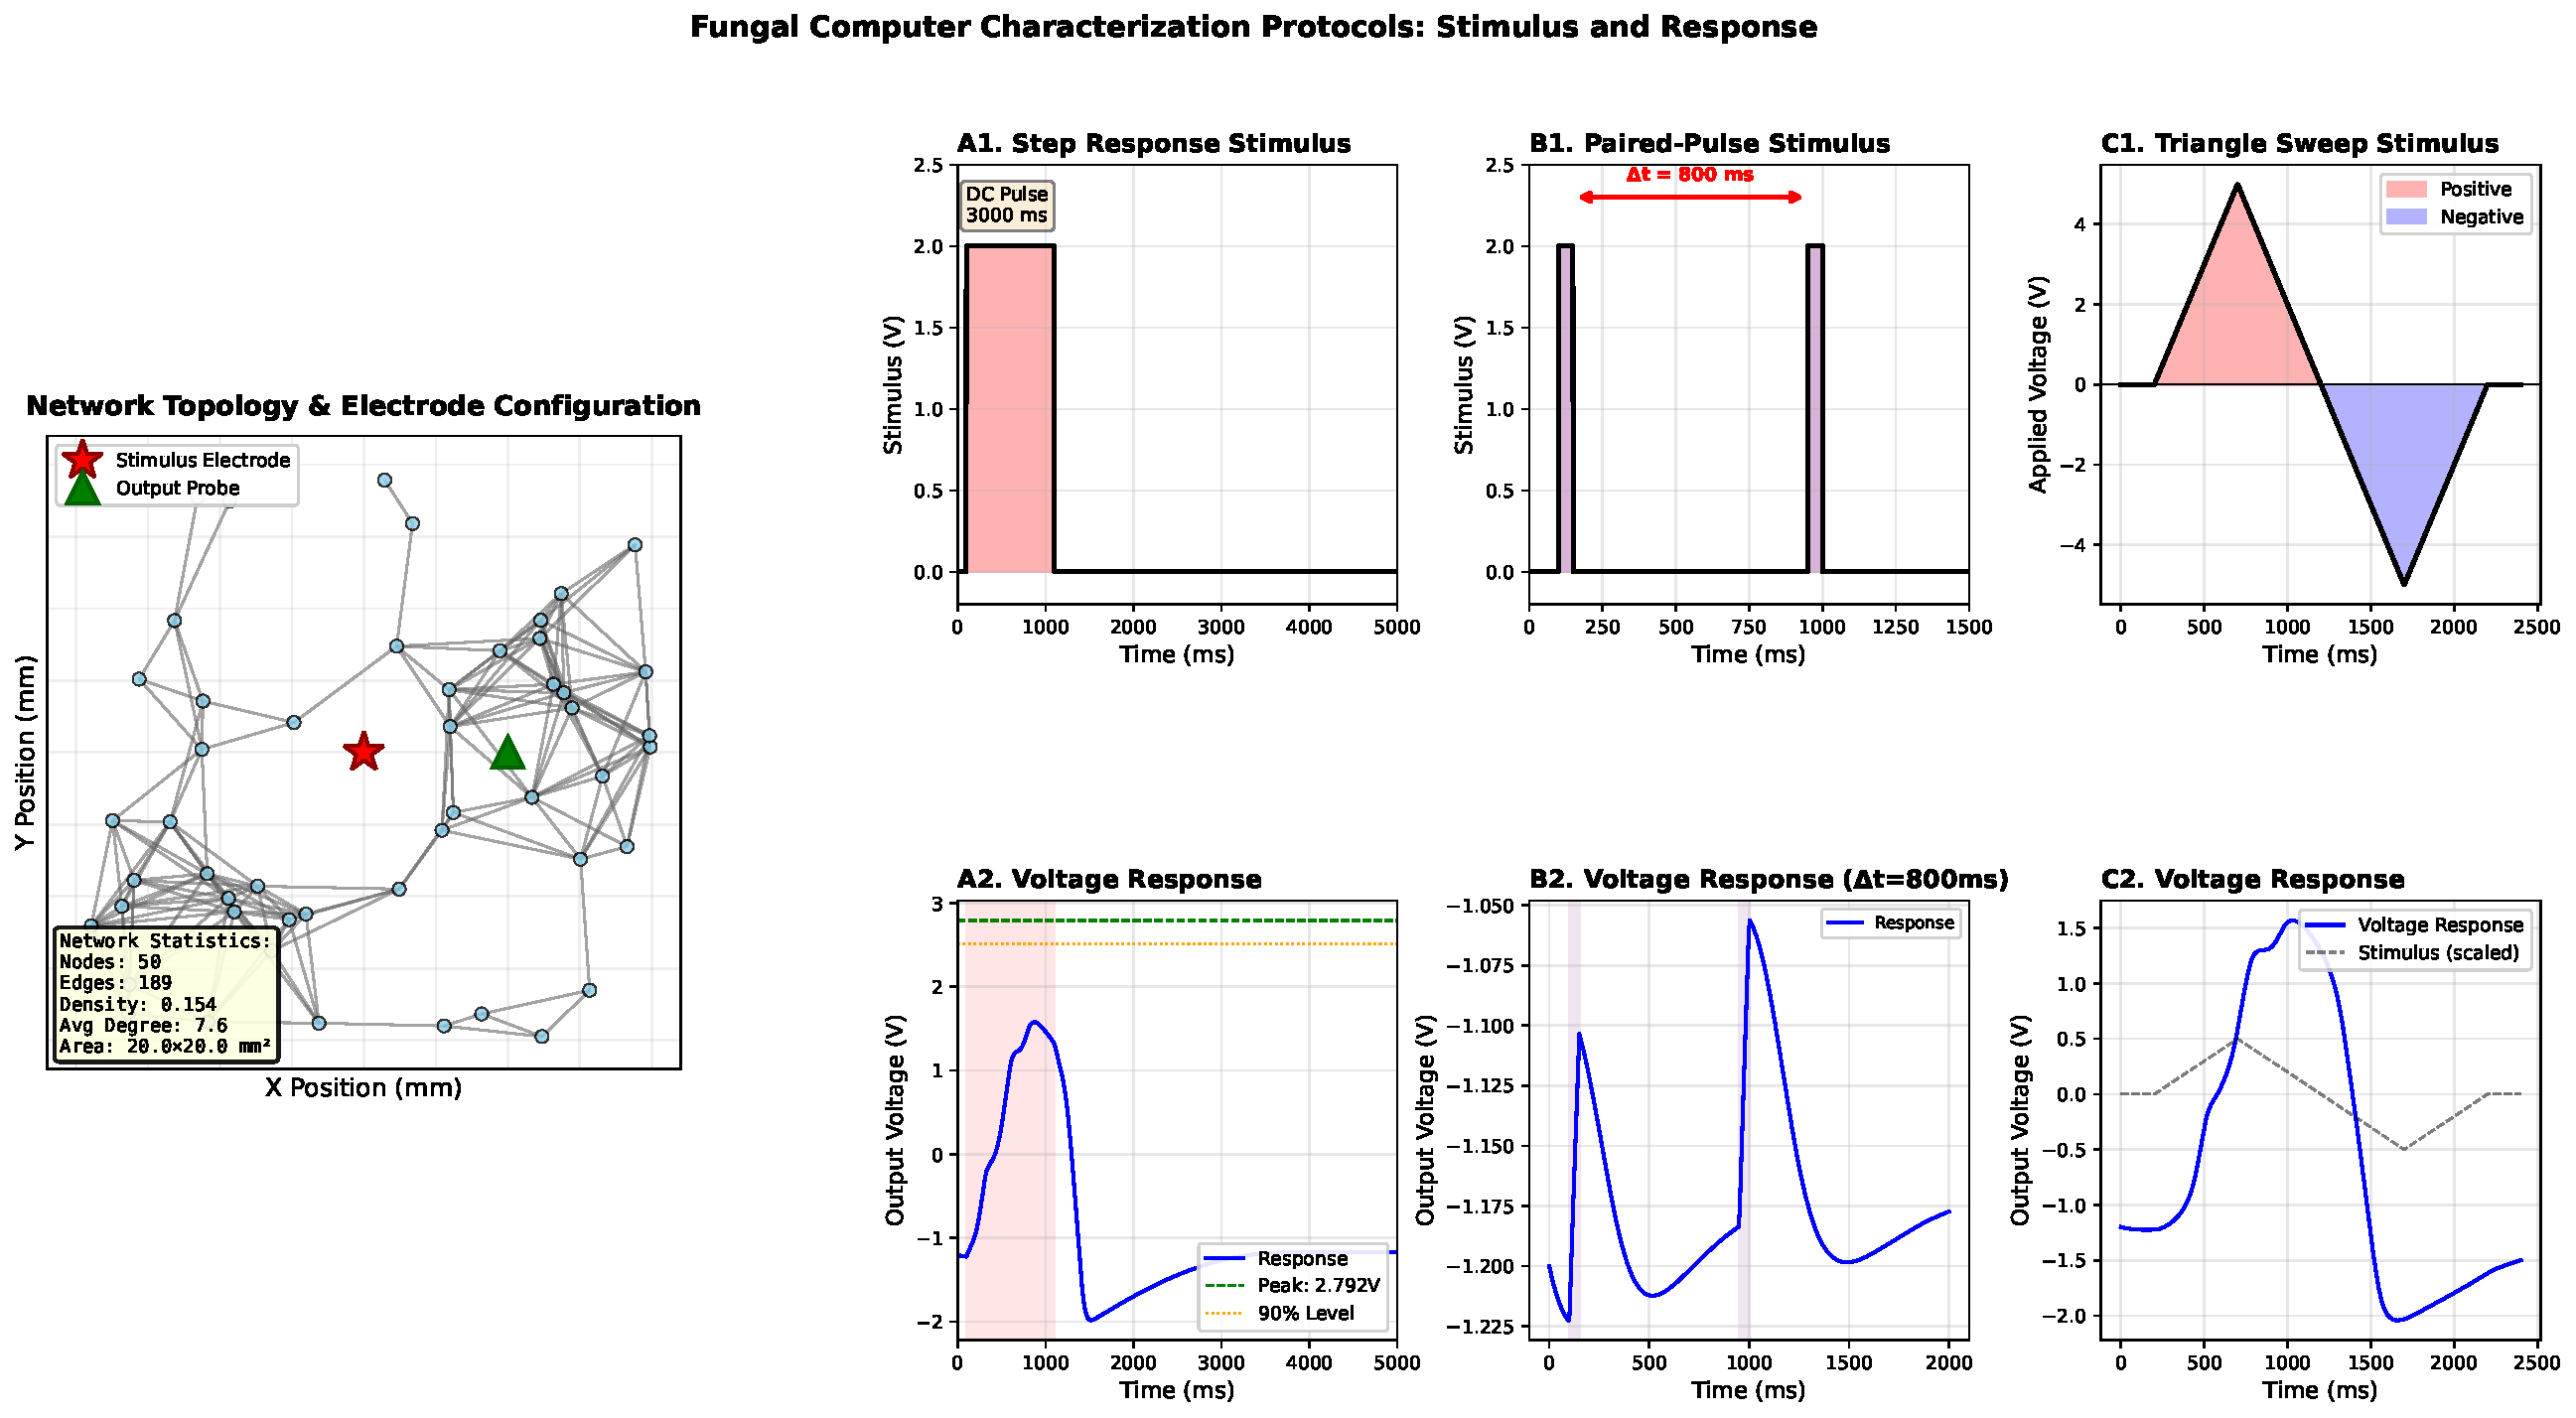
\includegraphics[width=0.99\textwidth]{figures/fig_characterization_protocols.pdf}
\caption{Characterization protocols used to probe the fungal digital twin model. The left panel shows a representative network and stimulation geometry; the right panels illustrate the step-response, paired-pulse, and triangle-sweep protocols and the types of waveform statistics extracted from each response.}
\label{fig:characterization}
\end{figure*}

\subsection{Parameter Prediction and Ablation}
We trained separate regressors for each target parameter using the 94-dimensional feature vectors. Two model families were compared: random forests and multilayer perceptrons. Performance was measured on a held-out 20\% test split using $R^2$ and RMSE. Because the goal is not only prediction but also experimental design, we also ran a protocol ablation study in which models were retrained on subsets of the feature set (step only, paired-pulse only, triangle only, and their pairwise combinations). This isolates which protocol families contribute information about which latent parameters.

\subsection{Reduced Rediscovery Validation}
A reduced rediscovery script has been prepared for the camera-ready version. It evaluates only three conditions on pre-optimized specimens: oracle parameters, direct ML prediction, and ML followed by waveform-matching refinement. The reported metrics are restricted to per-parameter estimation error and waveform mismatch; no XOR transfer claims are made in this paper. Because that run is still in progress, the corresponding result figure is left as a placeholder.

\section{Results}
\subsection{XOR Viability Occupies a Constrained Region of Parameter Space}
The systematic optimization study completed 160/160 runs successfully. Defining viability as the top quartile of tuned XOR scores yielded 40 viable specimens with threshold $0.0627$. Viable specimens appeared across the full range of graph sizes, but the highest-scoring subset was somewhat enriched in the larger networks (100--120 nodes). This suggests that larger graphs may increase the chance of high-performing specimens, even though XOR viability is not confined to one narrow topological regime.

\begin{figure}[t]
\centering
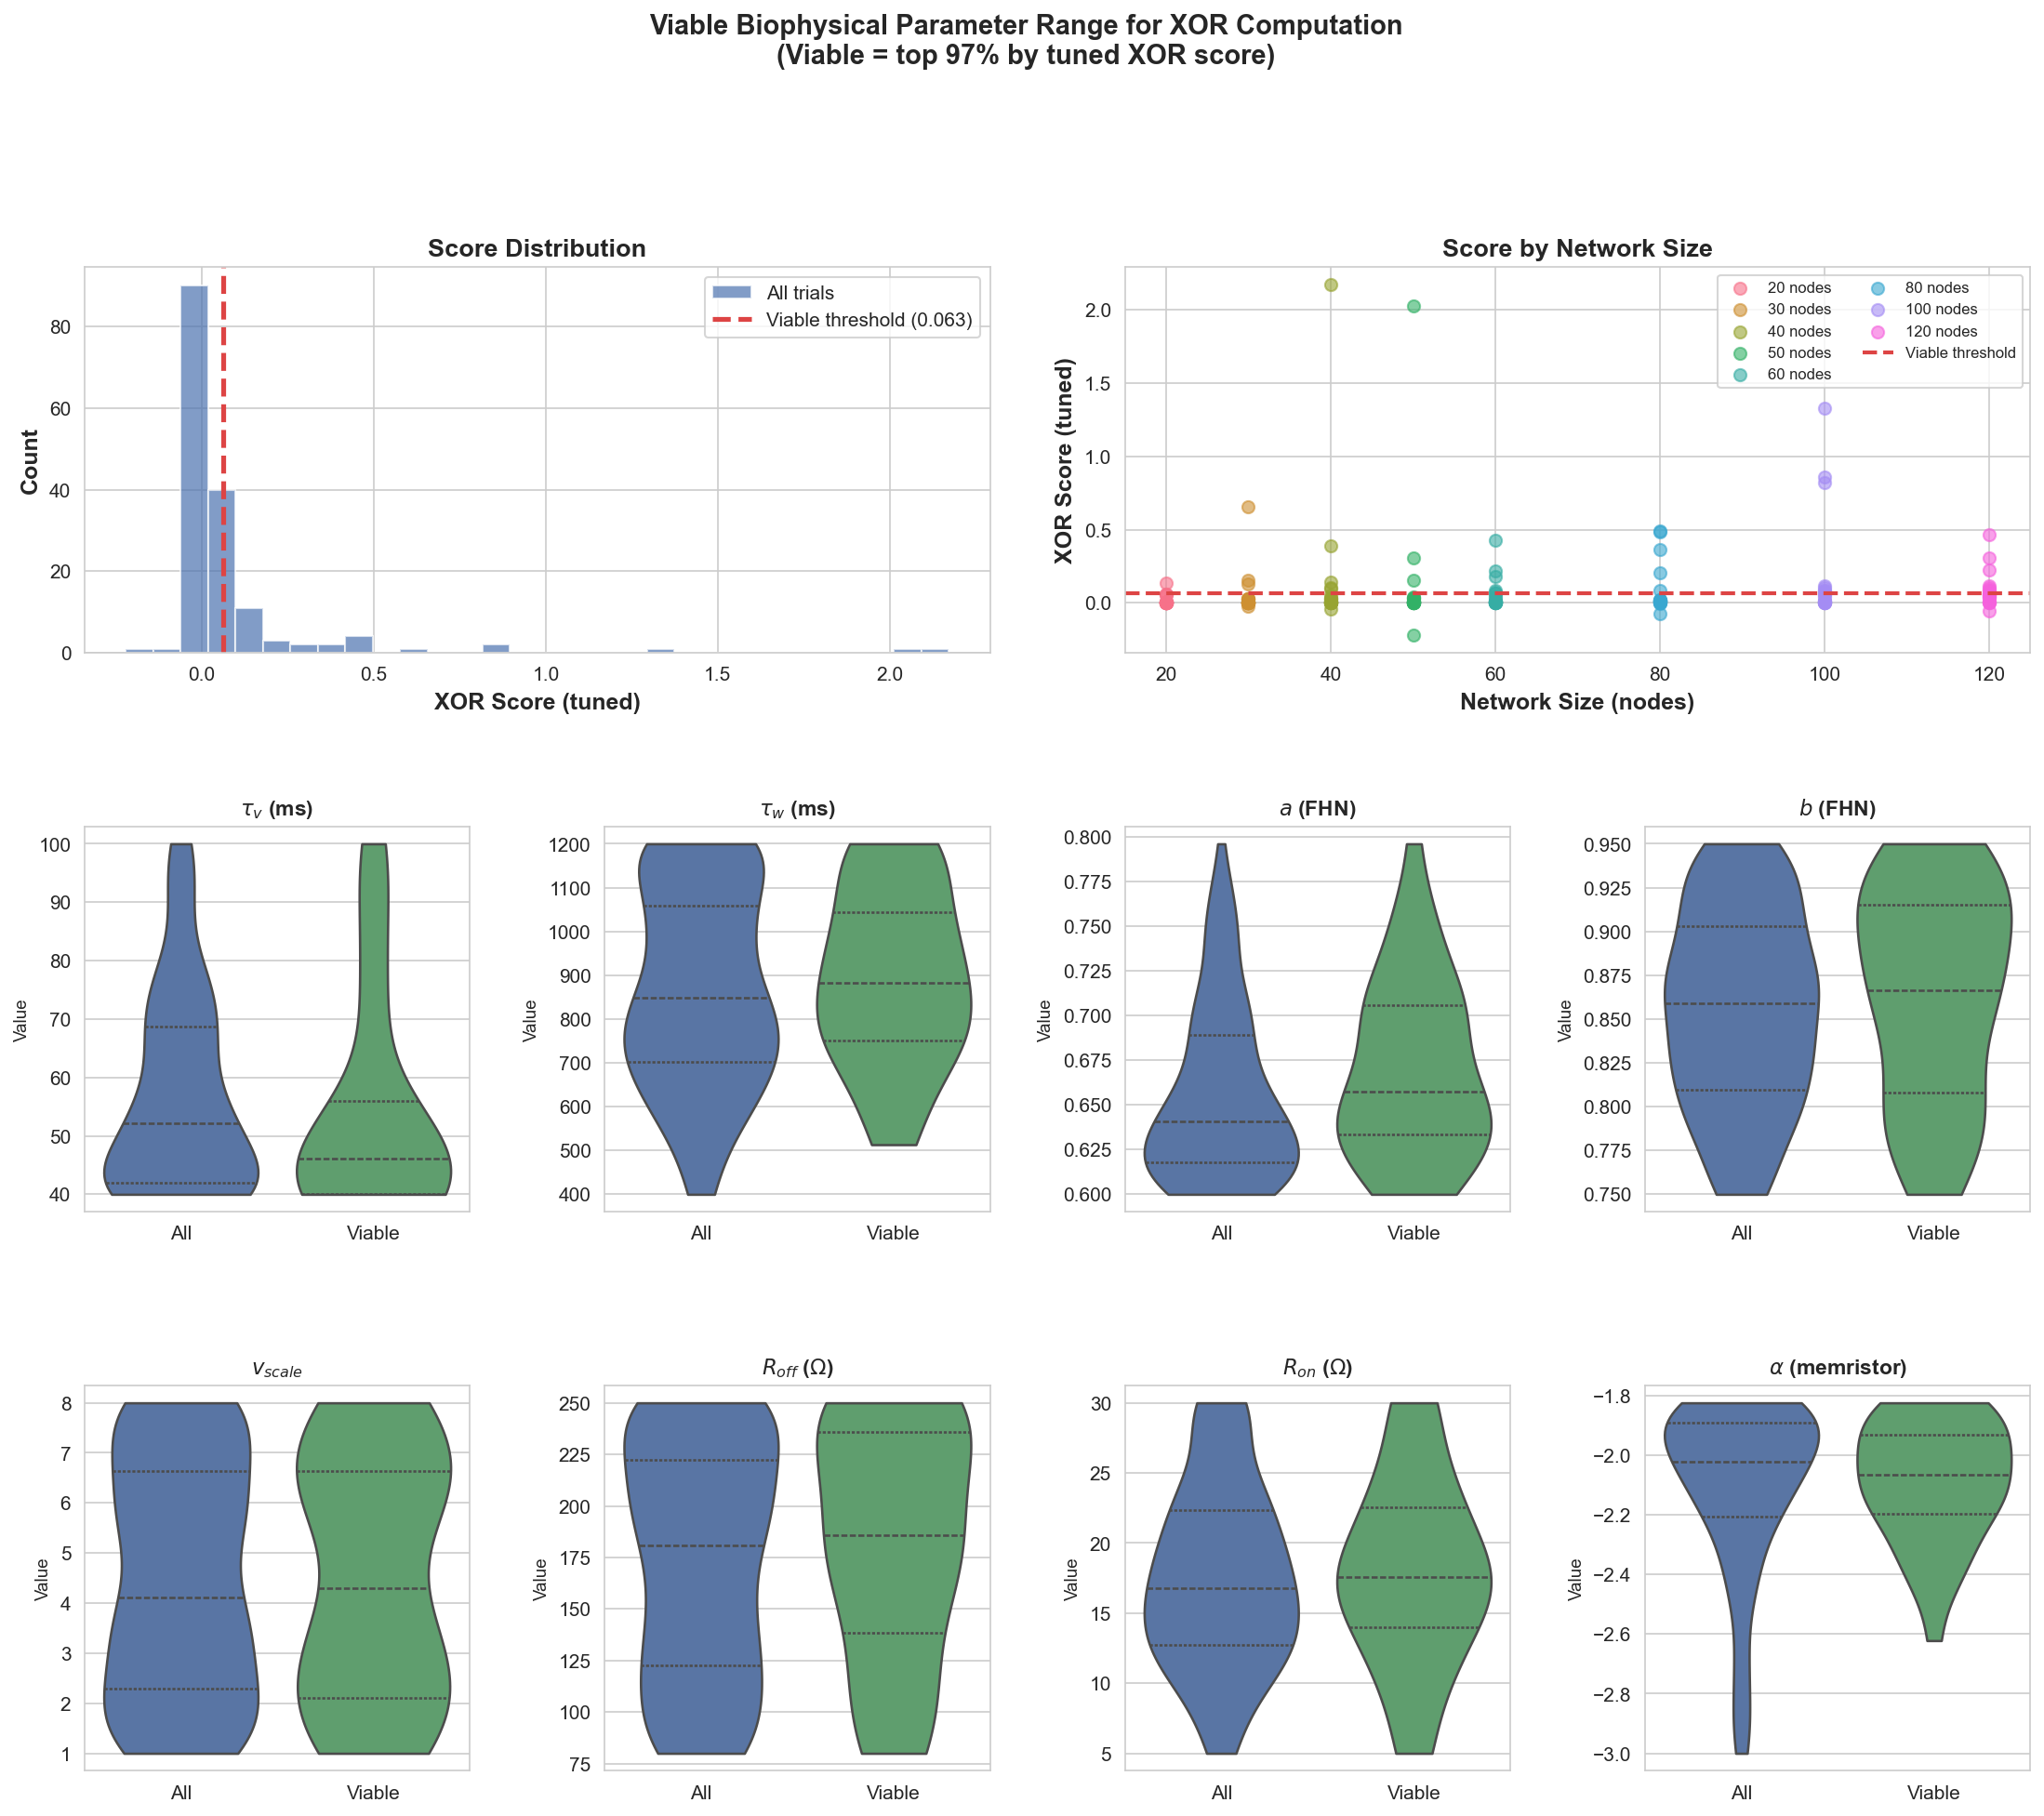
\includegraphics[width=\columnwidth]{figures/fig_viable_range.png}
\caption{Distribution of tuned XOR scores and tuned parameter values for all optimized specimens versus the top quartile of viable XOR substrates. Viable specimens occupy a narrower parameter region than the full search space, providing a computational prior for subsequent identification studies.}
\label{fig:viable}
\end{figure}

\Cref{fig:viable} summarizes the viable region. Compared to the full search bounds, the viable subset concentrates around $\tau_v \approx 54$, $\tau_w \approx 894$, $a \approx 0.67$, $b \approx 0.87$, $R_{\mathrm{off}} \approx 182$, $R_{\mathrm{on}} \approx 17.9$, and $\alpha \approx 0.009$. The viable subset also exhibited characteristic stimulation geometry: input electrodes were separated by $7.8 \pm 6.4$~mm, while the mean input-to-output distance was $13.1 \pm 3.5$~mm; mean voltage was $2.71 \pm 0.91$~V and pulse duration $2869 \pm 1634$~ms. Importantly, several viable parameter marginals were multimodal, indicating that XOR-supporting fungi are better interpreted as a family of dynamical regimes than as a single optimal point.

\subsection{Electrical Probes Recover Some Parameters Reliably but Not All}
All 400 characterization simulations completed successfully. The resulting dataset supported accurate recovery of a subset of the latent parameters. Random forests clearly outperformed multilayer perceptrons and were therefore used in all downstream analyses.

\begin{table}[t]
\centering
\caption{Held-out random forest performance overall and within each parameter's viable interval. Viable intervals are taken from the XOR-viable range analysis. Lower viable-range $R^2$ values should be interpreted carefully because the target variance is smaller inside a restricted interval.}
\label{tab:ml}
\small
\begin{tabular}{lrrrrr}
\toprule
Parameter & Overall $R^2$ & Overall RMSE & Viable $n$ & Viable $R^2$ & Viable RMSE \\
\midrule
$\tau_v$ & 0.912 & 10.566 & 37 & 0.746 & 8.857 \\
$\tau_w$ & 0.816 & 145.757 & 58 & 0.730 & 127.935 \\
$a$ & 0.717 & 0.044 & 47 & 0.065 & 0.047 \\
$b$ & 0.342 & 0.068 & 63 & 0.210 & 0.056 \\
$v_{scale}$ & -0.007 & 2.501 & 71 & -0.031 & 2.218 \\
$R_{off}$ & -0.244 & 81.195 & 62 & -0.196 & 63.808 \\
$R_{on}$ & 0.017 & 13.538 & 39 & -1.340 & 12.259 \\
$\alpha$ & 0.396 & 0.003 & 30 & -0.038 & 0.004 \\
\bottomrule
\end{tabular}
\end{table}

The strongest global predictions were for the two time constants and the excitability threshold: $R^2=0.912$ for $\tau_v$, $0.816$ for $\tau_w$, and $0.717$ for $a$ (\Cref{tab:ml}). Parameter $b$ was only moderately predictable ($R^2=0.342$), while $\alpha$ was weak but still above chance ($R^2=0.396$ with small absolute RMSE but large relative error because the parameter spans a small numerical range). In contrast, $v_{\text{scale}}$, $R_{\mathrm{on}}$, and $R_{\mathrm{off}}$ were not recovered reliably from the present protocols. This is an important negative result: the current stimulation set is sufficient for partial, not complete, identifiability.

Breaking performance out by viable interval clarifies how these predictors behave where XOR is actually relevant. Absolute RMSE within the viable interval is similar to or lower than the overall RMSE for six of the eight parameters, including $\tau_v$, $\tau_w$, $b$, $v_{\text{scale}}$, $R_{\mathrm{off}}$, and $R_{\mathrm{on}}$. However, viable-range $R^2$ is often lower than overall $R^2$ because the viable subset occupies a narrower slice of parameter space. In practice this means the models can still be locally useful within the viable regime even when variance-explained statistics deteriorate under range restriction. The clearest examples are $\tau_v$ and $\tau_w$, which retain both low viable-range RMSE and substantial viable-range $R^2$.

\begin{figure*}[t]
\centering
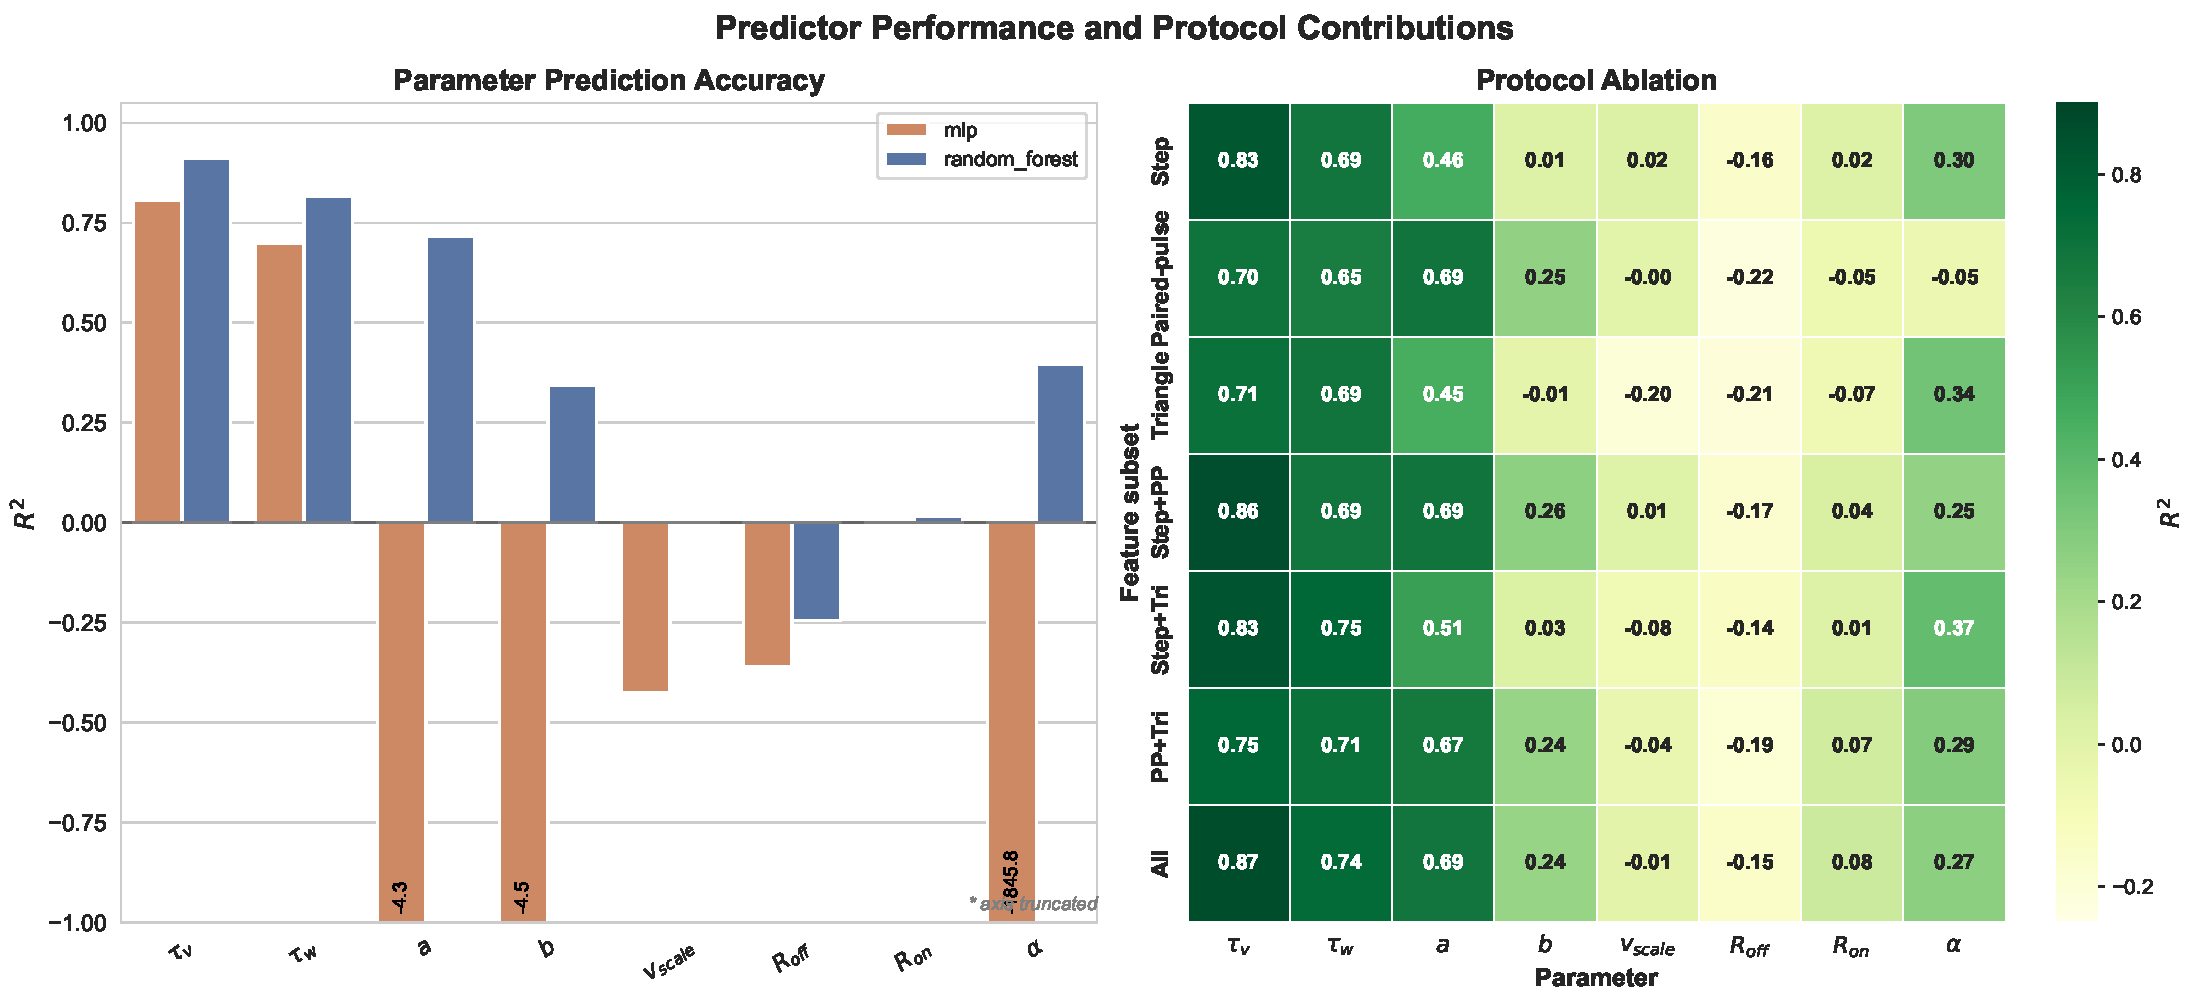
\includegraphics[width=0.98\textwidth]{figures/fig_prediction_ablation.pdf}
\caption{Left: held-out $R^2$ for random forest and MLP predictors across the eight biophysical parameters. Right: protocol-ablation heatmap showing how prediction quality depends on which characterization protocols are included.}
\label{fig:prediction_ablation}
\end{figure*}

\subsection{Different Protocols Capture Different Latent Dynamics}
Protocol ablation reveals a consistent division of labor across the stimulation set (\Cref{fig:prediction_ablation}). The full 94-feature model gave the best overall mean performance, but no single protocol dominated every target. Step response features carried most of the information for $\tau_v$. Paired-pulse features were most informative for $a$, indicating that short-timescale recovery and facilitation are especially diagnostic of the excitation threshold. The combination of step response and triangle sweep was best for $\tau_w$, $\alpha$, and $R_{\mathrm{off}}$, suggesting that slower recovery and memristive properties are better exposed by combining transient and hysteretic probes. Parameters $v_{\text{scale}}$ and the resistance pair remained difficult across all ablations, reinforcing the interpretation that the present protocol library underconstrains those aspects of the model.

\subsection{Reduced Rediscovery Validation Placeholder}
The reduced rediscovery section will report waveform mismatch and parameter error for oracle, ML-only, and ML-refined twins on a small set of pre-optimized specimens. The relevant script is prepared and running, but the results are intentionally excluded from this draft to avoid overclaiming. The placeholder figure is shown in \Cref{fig:rediscovery_placeholder}.

\begin{figure}[t]
\centering
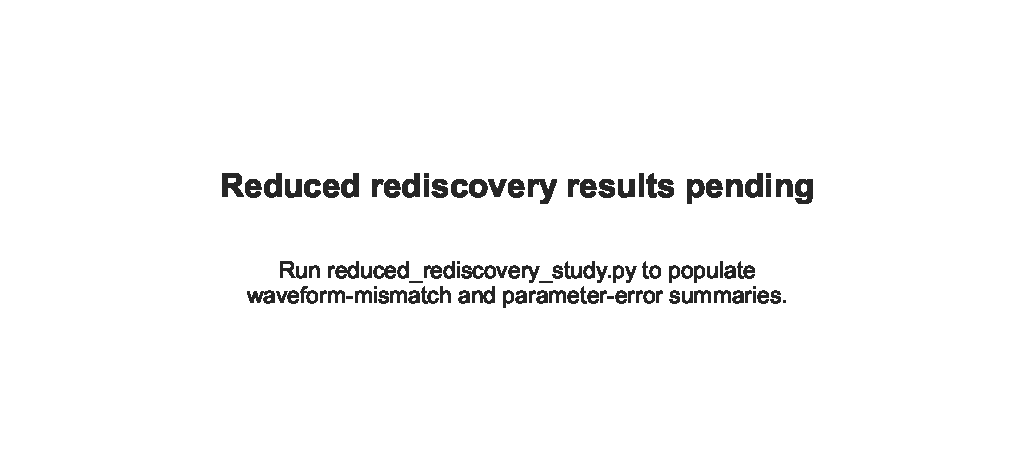
\includegraphics[width=\columnwidth]{figures/fig_reduced_rediscovery_placeholder.pdf}
\caption{Placeholder for the reduced rediscovery validation. The camera-ready version will summarize waveform mismatch and parameter estimation error for oracle, ML-only, and ML-refined twins.}
\label{fig:rediscovery_placeholder}
\end{figure}

\section{Discussion}
The main result of this paper is that fungal digital twins are already useful at two levels relevant to ALIFE: they can discover viable computational regimes, and they can partially infer the hidden excitable and plastic dynamics that make those regimes possible. The first result is about substrate discovery. Rather than searching blindly over all fungal-like dynamics, the optimization study identifies a viable XOR-supporting subspace. The second result is about identifiability. Standardized electrical probes contain enough information to recover some latent parameters reliably, especially the dynamical time scales and the main excitability threshold.

This supports a specific view of fungal computing as an artificial-life problem. The fungal substrate is not simply a noisy implementation target for predefined circuits. It is an adaptive physical medium whose computational affordances depend on the interaction of topology, excitability, and plasticity. The digital twin is therefore valuable not because it perfectly reproduces every specimen, but because it narrows the design space to regions where useful behavior is likely and tells us which hidden variables can be inferred from experimentally accessible probes.

The negative results are equally important. Three parameters ($v_{\text{scale}}$, $R_{\mathrm{on}}$, $R_{\mathrm{off}}$) are poorly constrained by the present protocol suite. This indicates a mismatch between what the model treats as important and what the current probes actually observe. For ALIFE this is not a weakness of the paper; it is part of the contribution. The ablation study shows how protocol design and identifiability are coupled, and it suggests where future empirical effort should focus: richer hysteretic sweeps, stronger perturbations of conductance-dependent dynamics, or explicitly multi-electrode identification protocols may be needed to resolve the resistance-related parameters.

There are also two important limitations. First, the current ML dataset samples the full parameter box rather than only the viable XOR subspace. This means the predictor is trained for broad coverage rather than task-specific identification. That choice is appropriate for the present paper because it establishes baseline identifiability across the whole model family, but a viable-range-conditioned dataset is a logical next step. Second, the reduced rediscovery validation is not yet complete, so this paper deliberately stops short of claiming robust functional transfer of optimized XOR gates back to unknown specimens. That stronger end-to-end claim belongs in the journal extension.

The viable-range analysis adds one more nuance to that limitation. Evaluating predictors inside the XOR-relevant intervals does not uniformly improve $R^2$, but it often improves or preserves RMSE. This is exactly what one would expect under range restriction: once the task becomes local calibration rather than global coverage, absolute error is the more informative metric. For the next stage of the project, it would therefore be sensible to report both variance-based and scale-based error measures when training specifically on the viable subspace.

Taken together, the results motivate a staged research program. An ALIFE contribution can reasonably center on viable-regime discovery, protocol-based identification, and the design of digital twins as exploratory models for living computation. A fuller Natural Computing paper can then extend the present work with completed waveform-refinement experiments, viable-range-conditioned retraining, and a direct evaluation of whether calibrated twins are good enough to support specimen-specific gate fabrication.

\footnotesize
\bibliographystyle{apalike}
\bibliography{example}

\end{document}
